%%%%%%%%%%%%%%%%%%%%%%%%%%%%%%%%%%%%%%%%%
% Dissertation Proposal
% 2017SoE027
% 
% Author: bmarron
% Origin: 27 Feb 2017
% Final:
%
% For a stand-alone doc:
% Insert contents into "Stand-Alone_template.tex"
%%%%%%%%%%%%%%%%%%%%%%%%%%%%%%%%%%%%%%%%%

%----------------------------------------------------------------------------------------
%	PACKAGES AND OTHER DOCUMENT CONFIGURATIONS
%----------------------------------------------------------------------------------------
\documentclass[reqno,12pt,oneside]{report}  % right-side equation numbering, 12-pt, print one-sided 

\usepackage{rac2}                          % Use "rac1" for thesis; "rac2" for thesis proposal (fr. Univ. of Michigan thesis template)
\usepackage{amsfonts}
\usepackage{amsxtra}                       % Use various AMS packages
\usepackage{graphicx}                      % Add some packages for figures. Read epslatex.pdf on ctan.tug.org
\usepackage{rotating}
\usepackage{color}
\usepackage{epsfig}
\usepackage{acronym}                       % For the List of Abbreviations. Read acronym.pdf on ctan.tug.org
\usepackage{setspace}                      % Allows you to specify the line spacing
\usepackage{outlines}                      % outlines
\usepackage{lipsum}                        % Package to generate dummy text throughout this template
\usepackage{csquotes}
\usepackage[natbibapa]{apacite}
\usepackage[english]{babel}
\usepackage{amsmath}
\usepackage{amsthm}
\usepackage{amssymb}
\usepackage{pdfpages}
\usepackage{verbatim}
\usepackage{bigfoot}
\usepackage{multirow}
\usepackage{booktabs}                                 % Horizontal rules in tables
\usepackage{float}                                    % place Tables/Figs in specific locations with the [H] (e.g. \begin{table}[H])
\usepackage{paralist}                                 % makes bullet points with less space between them
\usepackage[sc]{mathpazo}                             % Use the Palatino font and the Pazo fonts for math
\usepackage{microtype}                                % Slightly tweak font spacing for aesthetics
\usepackage[hmarginratio=1:1,top=32mm]{geometry}      % Document margins
\usepackage[hang, small,labelfont=bf,up,textfont=it,up]{caption} % Custom captions 

\usepackage{xspace}
\let\OldS\S
\renewcommand{\S}{\OldS\xspace}

\usepackage{draftwatermark}
\SetWatermarkLightness{0.95}
\SetWatermarkScale{1}


\renewcommand\labelitemi{{\boldmath$\cdot$}}          %medium bullets
%\renewcommand\labelitemi{$\cdot$}                    %small bullets


\usepackage[T1]{fontenc}                              % Use 8-bit encoding that has 256 glyphs
\linespread{1.05}                                     % Line spacing - Palatino needs more space between lines
\onehalfspacing                                       % \onehalfspacing for 1.5 spacing, \doublespacing for 2.0 spacing.



\usepackage{abstract}                                       % Allows abstract customization
\renewcommand{\abstractnamefont}{\normalfont\bfseries}      % Set the "Abstract" text to bold
\renewcommand{\abstracttextfont}{\normalfont\small\itshape} % Set the abstract itself to small italic text


%-------------------------------------------------------------
% NEW COMMANDS
%---------------------------------------------------------------------
%This command creates a box marked ``To Do'' around text.
%To use type \todo{  insert text here  }.
\newcommand{\todo}[1]{\vspace{5 mm}\par \noindent
\marginpar{\textsc{To Do}}
\framebox{\begin{minipage}[c]{0.95 \textwidth}
\tt\begin{center} #1 \end{center}\end{minipage}}\vspace{5 mm}\par}


\newcommand{\sun}{\ensuremath{\odot}} % sun symbol is \sun


% To use paragraph indents
%\begin{myindentpar}{2em}
% blah blah blah
%\end {myindentpar}
\newenvironment{myindentpar}[1]%
   {\begin{list}{}%
       {\setlength{\leftmargin}{#1}}%
           \item[]%
   }
     {\end{list}}


%-----------------------------------------------------------------
% START DOCUMENT
%-----------------------------------------------------------------
\begin{document}

\titlepage{The Ecological Assessment of Agroecological Landscapes for Sustainable Cropping Systems}{Bruce D. Marron}{Doctor of Philosophy}{Earth, Environment, and Society}{2017}
{$\checkmark $ Dr. Robert Scheller, Prof. of Environmental Science \\
 Dr. Michelle , Asst. Prof. of Agroecology\\
 Dr. J. Arturo Maldonado, Assoc. Professor of Agroecology\\
 }


%-----------------------------
% FRONT SECTIONS
%------------------------------

\initializefrontsections

% Optional: Frontispiece graphic/text
\frontispiece{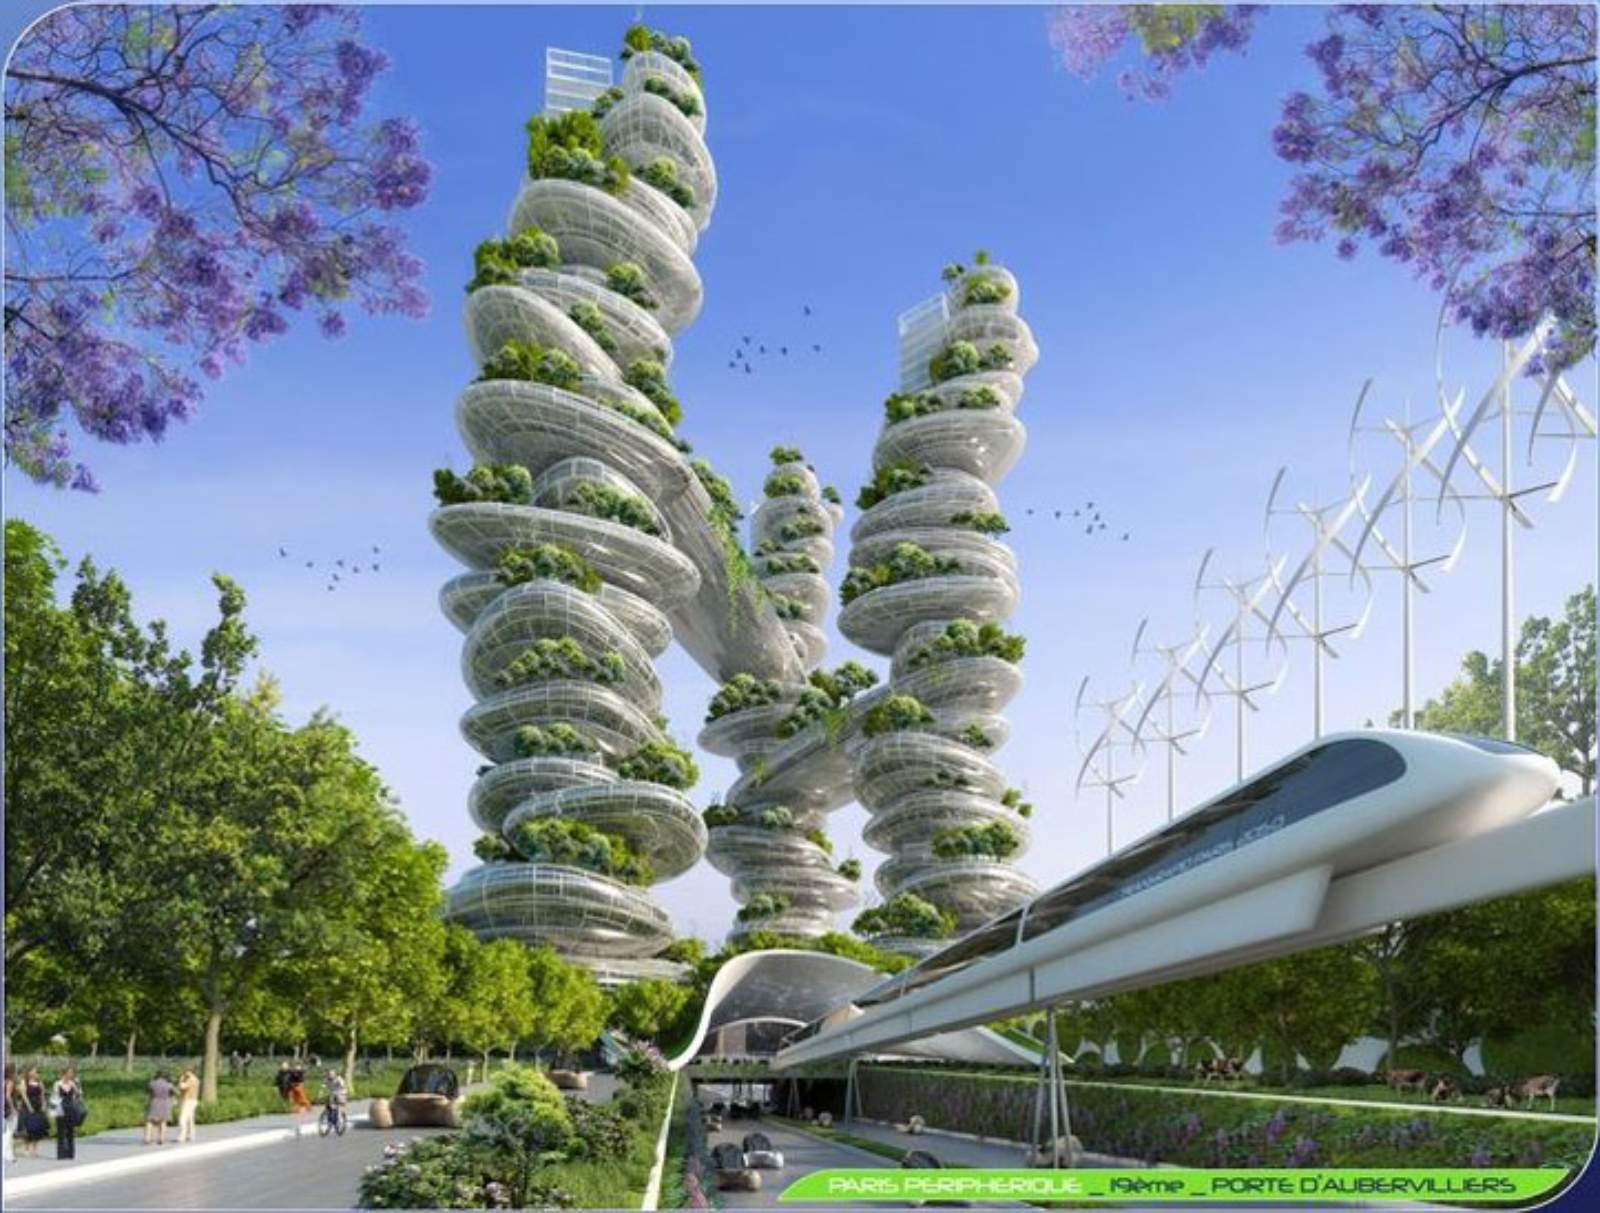
\includegraphics[width=6in]{FrontSections/fig1c} Paris, 2050}

% Optional: Copyright page
%\copyrightpage{Bruce D. Marron}

% Optional: Dedication page
%\dedicationpage{To all of the two-foots, four-foots, and no-foots\\
% \todo{ More to add here!!}}

% Optional: Acknowledgements page
%\startacknowledgementspage
%Thanks to the people who made this dissertation possible, especially those who put together a nice \LaTeX\, template for me to use.
%\label{Acknowledgements}

% Optional: Preface page
%\startprefacepage
%\input{Preface}
%\label{Preface}


%----------------------------------------------------
% TABLE OF CONTENTS
%----------------------------------------------------


\tableofcontents                        % Required
\listoffigures                          % Required if there is more than one figure
\listoftables                           % Required if there is more than one table
\listofmaps                             % Required if there is more than one map
%\listofappendices                      % Required if there is more than one appendix
\listofabbreviations                    % Optional. Abbreviations should be stored in a file named abbr.tex


%----------------------------------------------------------
% (In-Dissertation) ABSTRACT
%----------------------------------------------------------

%\startabstractpage
%{The Title of Your Dissertation}{Your Name}{Chair: Albert Einstein}
%\textit{This template conforms to University of Michigan abstract and dissertation format guidelines as of September 2008. It is an update to a template that has been floating around among grad students here for about 20 years. The main components are the thesis.tex file and the rac.sty file, the latter of which should not need any modification. If BibTeX is used (and for a dissertation, it should be), then References.bib is also needed. If a list of acronyms is desired, make all additions in abbr.tex and read acronym.pdf on ctan.org for details on how to call them in the text. Other files in this template that may be helpful, but don't necessarily need to be used include a style file that formats your bibliography in AGU format (agu04.bst) and a style file that allows you to use abbreviations for journal names (aas\_macros.sty) when typing out the bibliography. This will be necessary if you grab BibTeX information from places like the NASA ADS, which sometimes uses journal name abbreviations. It is useful to separate chapters into their own subfolders, with each folder containing the chapter's .tex file as well as all associated figures. For the figures, just call the name of the file, without the suffix (i.e., includegraphics\{Chap5/LabSetup\}) and the graphicx package will figure out what type of file it is. To compile to pdf, some format other than .eps must be used with the figures. To compile to ps, the figures need to be in ps or eps. If using \LaTeX\, in a Windows environment, there are several different editors and programs that can be used. One set that is known to work well is the following, which can each be found with a simple web search and which should be installed in this order: a Perl distribution such as ActivePerl, a \TeX\, distribution such as MikTex, a \LaTeX\, editor such as TeXnicCenter, a postscript interpreter like Ghostscript, and a postscript viewer like GSView. I included a few pages of sample code in chapter 2 to help you get started, including code for writing equations, citations, abbreviations, tables, and calling graphics. Always be sure to compile your thesis.tex file a couple of times to get the references and page numbering updated.} Good luck. -jg

%\label{Abstract}


%--------------------------
% CHAPTERS
%---------------------------

\startthechapters 
% The individual files for each of the chapters are put here.
% Save each chapter to a separate tex file and then use the 
%"\input{}" command to include this file. 
 
  
\chapter{A Complex Problem}
 \section{Introduction}
Will it be possible to feed ourselves over the next 50 years without crashing the biosphere? This is a pressing and complex problem. Even without social and political considerations, a variety of physical and ecological feedback mechanisms are currently operating in coupled human and natural systems at both global and national scales that are expected to place severe constraints on the national and regional production of ecosystem goods and services as early as 2050 \citep{zhao_drought-induced_2010, hoegh-guldberg_impact_2010, eigenbrod_impact_2011}. Ultimately, the outcomes of climate change (including ocean acidification, sea level rise, drought, shifts in storm regimes) the demands of economic growth (including increased natural resource extraction, pollution, appropriation of natural land area), and the surge of a human population to 9 billion are the drivers fueling these detrimental feedback mechanisms. Of perhaps greatest concern among those ecosystem service outputs threatened with decline are the two fundamental to human existence; namely, freshwater and food \citep{dodds_human_2013, rogers_facing_2008, lobell_climate_2011, wada_global_2010, zhao_drought-induced_2010, schmidhuber_global_2007, tilman_forecasting_2001, tilman_agricultural_2002}. 

Over the coming decades, agricultural production systems, which are already facing relentless competition for land, water, and energy, will be expected to deliver increasing amounts of diverse, highly-nutritious foods (especially animal-derived products) to an increasingly affluent global population while simultaneously (a) reducing the environmental externalities of production, (b) reducing impacts to natural biodiversity, (c) boosting crop biodiversity, (d) improving the social justice of food access, (e) adapting to shifting climates, intense weather events, and higher carbon dioxide levels, and (f) remaining economically viable in a globalized economy. Optimizing under this suite of constraints will require more than simply maximizing short-term yields. It will require a tremendous shift in agricultural practices to agroecology-based agronomic design principles with the long-term goals of sustainable yield, increased soil fertility, increased soil organic carbon, increased aboveground and belowground biodiversity, and increased transpiration efficiency. 

The research program presented in this document uses the theoretical constructs and metrics of contemporary, soil biota-based, agroecology coupled with (a) spatially-explicit ecological processes and (b) natural disturbance regimes to develop scenario-based, simulation modeling tools and probability-based inference tools for evaluating the ecological robustness, resiliency, stability, and adaptability of various cropping system design patterns at the regional (landscape) scale over time. The aim of the proposed research program is to hasten the successful transition to sustainable food production systems and enhance regional biodiversity by (a) defining sustainable agriculture as a set of agroecological mutualisms brokered by functional soil foodweb dynamics, (b) using the scenario-based, simulation modeling tools and probability-based inference tools to design spatially-explicit agroecological patterns that can enhance and maintain soil fertility and agricultural productivity over time, and (c) providing academic researchers as well as decision makers (agriculturists, land use planners, and agricultural policy makers) with accessible, science-based tools for the ecological assessment of agroecological landscapes. 

To be realized, sustainable agriculture must be defined by more than "bucket lists" of desiderata (see Appendix A). The proposed research program seeks to identify the necessary and sufficient ecological conditions to establish patterns of sustainable agriculture on a given landscape by linking aboveground productivity to the biodiversity of belowground  soil biota through the processes mediated by functional soil food webs. 

\section{The Harsh Realities of Modern Industrial Agriculture}
\begin{comment}
Current industrial agricultural practices jeopardize economic, ecological, and social sustainability and the long-term delivery of ecosystem goods and services. Economic sustainability, whether 'strong' or 'weak', relies on natural capital as the source for both primary and manufactured goods. Any substantial reduction in natural capital therefore reduces economic opportunity and potentially points to a decline in future human welfare \citep{pearce_blueprint_2000}. If the endowment of natural capital required for ecosystem goods and services is taken as the aggregate of functional terrestrial and aquatic ecosystems across the globe, then industrial agricultural reduces natural capital through loss of topsoil, creation of oceanic hypoxic zones, damage to hydrological systems, disruption of soil foodwebs, destruction of natural habitats across multiple scales, production of greenhouse gases, and loss of genetic diversity \citep{gliessman_agroecology:_2015}. Collectively these are externalized costs that result from (a) failure to properly value ecosystem goods and services, (b) failure to account for the true costs of environmental degradation and natural capital depletion, and (c) failure of markets and policies to provide incentives for sustainable stewardship of natural capital \citep{pearce_blueprint_2000}. 

\todo{provide additional discussion of environmental/ecological \\
externalities from industrial ag}
\begin{outline}[enumerate]
\1 Modern industrial agriculture negatively affects regional ecology and regional effects aggregate to disrupt global ecological functionalities.
\2 high algal blooms...
\2 Industrial ag is a primary source of anthropogenic inputs into natural biogeochemical cycles at the regional scale ... (the main inputs? the biogeochemical cycles of concern? the mechanisms and effects of inputs?)
\2 Industrial ag effects are aggregated to the global scale ... (mechanisms? examples?) 
\2 Regional inputs affect ecologies at a distance from source ... (mechanisms? examples?)
\2 The current state of worldwide ecosystem functionality is ... (examples? expectations?)
\end{outline}

Industrial agriculture likewise threatens environmental sustainability. Humans rely on a functional biosphere for life support and industrial agriculture's externalized costs are environmentally devastating at the global scale \citep{tilman_agricultural_2002, wolfe_crop_2000, ceballos_accelerated_2015}. To take but two of many quantitative examples, the anthropogenic sources of reactive nitrogen that are directly linked to agriculture (i.e., fertilizer production by N-fixation from the Haber-Bosch process and fertilizer production by N-fixation from cultivation) now contribute reactive nitrogen to the biosphere at nearly double the rate of terrestrial nitrogen fixation (i.e., at about $13 \ x \ 10^{12} \ mol \ yr^{-1}$) \citep{canfield_evolution_2010}. And the agricultural sector is the third largest contributor of greenhouse gases behind transportation and power generation \citep{gliessman_agroecology:_2015}.

Finally, industrial agriculture can disrupt social sustainability. Confronted with industrial agricultural practices, rural agricultural communities may experience a loss of local control over agricultural production with a resulting loss in place-based knowledge, human capital, and civic engagement \citep{beus_conventional_1990, oecd_well-being_2001}. Recently concerns have been raised over the social costs of inequities in the final distribution of benefits and burdens associated with the production of ecosystem goods and services \citep{berbes-blazquez_towards_2016}.
\end{comment}

\section{A Compound Problem Statement}
The proposed research program considers three crucial elements of the complex problem of designing and assessing agroecological landscapes for sustainable cropping systems. The proposed research program uses a variant of the \enquote{decision-maker model} to identify, describe, and prioritize the three problem elements below \citep{gordon_planning_2007}. 

\subsection{Element 1}
\begin{comment}
\textit{A typology of soil microbe communities is required for evaluating the functional capacity of soil foodwebs. The typology must be capable of integrating field data from both in situ optical microscopy and modern genomics.} \\


for (a) evaluation of the functional capacity of soil foodweb dynamics, (b) evaluation of the productivity, diversity and composition of plant communities in relation to nature and extent of the aboveground to belowground linkages, (c) readily obtainable metrics that provide indicator metrics


\begin{outline}[enumerate]
\1 current typologies
\2 Functionally (ie using an ecological typology) 
\2 Taxonomically  (ie using monophyletic, paraphyletic, or polyphyletic designators)
\2 Spatially (with reference to soil horizons OR the rhizosphere OR both)
\1 soil fertility == a vector of measurements on soil structure and soil chemistry. soil structure a fxn of soil microbes
\1 numbers of genera, spp in soil
\1 use of chronosequences
\1
\end{outline}
\end{comment}

\subsection{Element 2}
\textit{Process-based, spatially-explicit modeling tools for evaluating the relationships, mechanisms, and spatio-temporal processes that link natural ecosystems to agricultural production systems are unavailable.} \\

Agriculture directly couples humans to natural systems through agricultural-ecological linkages of matter, energy, and information. Clearly, such linkages can be used to generate vicious cycles. But agricultural-ecological linkages may also engender virtuous cycles when agroecological principles of whole-system management are realized \citep{gliessman_agroecology:_2015}. Agroecological mutualism is a landscape-scale emergent property that offers the prospect of generating virtuous cycles to the benefit of both people and the biosphere. Agrocological mutualism is defined as the set of complex linkages and relationships that provide for mutually beneficial transfers of matter, energy, and information between the agriculturally- (anthropogenically-) organized and the naturally-organized components of a multi-functional landscape. If realized, agroecological mutualism would (a) maintain high, annual net primary productivity (ANPP) in both components, (b) enhance the robustness and resilience of both components, and perhaps most importantly (c) maintain the necessary biodiversity and adaptive capacity which serves as grist for the global evolutionary mill.  High ANPP implies closed nutrient and energy loops that trap greater amounts energetic and material flows across a landscape thereby creating eco-functional redundancies and building variety in system-level regulators via trophic level expansion \citep{ashby_introduction_1955}. Enhanced robustness and resilience implies diverse assemblages of aboveground flora and belowground soil biota that can drive the ecological processes and dynamics required for maximal energy capture. And necessary biodiversity implies that evolution (an information processing learning algorithm) can rapidly explore the enormous state space of possible patterns of biological form and function in order to provide adaptations (i.e., biologically \enquote{fit} organisms) in our epoch of dramatic global climate change and mass extinction \citep{ceballos_accelerated_2015}. The realization of agroecological mutualism is implicit in the bucket lists of sustainable agriculture (see Appendix A) and in the concepts and methodologies of agroecology \citep{gliessman_agroecology:_2015}. 

The necessary and sufficient conditions for realizing agroecological mutualism on any given landscape are uncertain. And it remains unclear how to spatially and temporally integrate agriculture into the natural world at the landscape scale so that the benefits of agroecological mutualism are realized. There are many reasons why this is so. For example, landscapes are spatially and temporally dynamic over multiple scales of both. The resultant heterogeneity consists of a panoply of scale-dependent and perception-dependent mosaics that result from the complex interactions of biological, physical, and social forces and fluxes \citep{turner_landscape_1989}. Unraveling the mechanisms responsible for the relationships between landscape patterns and ecological processes is difficult not only because of the complexities of interaction, but because experimentation and hypothesis testing at broad spatial scales must be done with models when extrapolation from small-scale experimentation is invalid. Ultimately, having agricultural components on a landscape adds additional complexities because of their inputs of matter, energy, and genetic information to the coupled, human-natural system.


\subsection{Element 3}
\begin{comment}
\textit{Applications... There is current evidence that And there is evidence from a past, \enquote*{natural experiment} in the Yucat\'{a}n Peninsula that agroecological mutualism, and hence sustainable agriculture, is directly related to spatio-temporal patterns on the landscape.}\\

The dynamic, managed mosaic created by the traditional agricultural practices of the Lowland Mayan in the Yucat\'{a}n Peninsula during their Classical Period (300-900 AD) may be an example of an as-yet, unexplained natural experiment in agroecological mutualism. The Lowland Mayan people maintained an average population density of 100-200 $persons \ km^{-2}$ throughout the entire Yucat\'{a}n peninsula of Mexico for at least 600 years during their Classic Period. At their peak, the Maya were feeding several million people \citep{gomez-pompa_lowland_2003} and densities in ancient cities such as Chunchucmil (about 2500  $persons \ km^{-2}$ ) and Tikal (about 3800 $persons \ km^{-2}$) were even greater than densities in comparable cities in the region today \citep{dahlin_reconstructing_2005, faust_maya_2001}.  After much debate and revision, the Lowland Mayan population data are now accepted in the literature. This raises many questions related to sustainable agriculture such as,
\begin{itemize}
  \item What were the practices that enabled the Classic Period Maya to successfully feed themselves for centuries in a tropical region that is poorly suited to agriculture?
  \item How were high levels of biodiversity sustained under such intensive agricultural production? 
  \item Why was there no severe ecosystem damage resulting from high population densities until the first part of the ninth century? (Note that while many hold up the Mayan Collapse as a classic example of ecological disaster, \citet{gomez-pompa_lowland_2003} and \citet{diamond_collapse:_2006} point to drought-fueled, political unrest as the most likely causes.)
  \item What are the mechanisms, dynamics, processes, and state variables responsible for this phenomenon and critically, are these mechanisms generalizable and portable to non-tropical regions of agricultural production?
\end{itemize}

The answers to these questions appear to lie in the relationships between agricultural disturbance and the biodiversity of soil biota, especially of bacteria and fungi. 
\end{comment} 

  \label{chap:Intro}

  
\chapter{Assumptions and Logic}
 \section{Research Program Assumptions}

The proposed research program is built on assumptions logically alloyed from the conceptualizations and theoretical considerations from a variety of disciplines through a broad swath of peer-reviewed literature \citep{ingham_interactions_1985}, \citep{maeder_soil_2002}, \citep{polis_food_1996}, \citep{van_der_heijden_unseen_2008}, \citep{lavelle_faunal_1997-1}, \citep{kladivko_tillage_2001}, \citep{doran_soil_2000-1}, \citep{bongers_nematode_1999}, \citep{brussaard_soil_1998}, \citep{coleman_peds_2008}, \citep{sackett_linking_2010}, \citep{kardol_how_2010},\citep{van_der_putten_empirical_2009}, \citep{bardgett_belowground_2014}, \citep{scheller_forest_2004}, \citep{williams_simple_2010}, \citep{fath_ecological_2007}, \citep{harte_maximum_2011}, \citep{gianinazzi_impact_1994}, \citep{eigen_hypercycle_1979}, \citep{nicolis_exploring_1989}. 

This section provides a brief narrative of those assumptions and logical connections. The following are synthetic (not analytic) statements taken as primary assumptions derived, in part, from the references listed above.


\begin{outline}[enumerate]
  \1 There are ecological functionalities which link agricultural components of landscapes to natural components of landscapes to create multi-functional landscape wholes.
  
  \1 Ecosystem goods and services can be conceptualized as emergent properties of multi-functional landscape systems.
  
  \1 Specific component subsystems must be present and the activation of many subsystem processes are likely to be threshold controlled by one or more Heaviside-like step functions (i.e., thresholds exist that turn processes on and off).

  \1 Plants are "super-organisms" composed of the autotroph and its rhizospheric symbionts. There are massive feedback loops between the autotroph and its symbionts governed by large numbers of biological transducers.
  
  \1 Rhizospheric symbionts are species-rich communities of fungi and bacteria that feed directly from plant root exudates. These fungi and bacteria form the mutualisms that are the basis for a soil's rhizospheric-based soil food web component.

  \1 The rhizospheric-based soil food web component is a set of species-rich communities of fungi, bacteria, protozoa, and nematodes. The rhizospheric-based soil food web component is linked to the soil's detritus-based soil food web component, likewise a species-rich set of communities of fungi, bacteria, protozoa, and nematodes. Together, these two individual food web components form one, reticulate and mutualistic whole (the soil food web) with highly complex topology and population dynamics.
  
  \1 Homogeneous trophic levels do not exist in soil food webs although temporal distance from photosynthetic carbon can define soil food web typologies: Rhizospheric-based communities are $10^{1} - 10^{3} \ s$ from photosynthetic carbon, detritus-based communities are $ > 10^{3} \ s$ from photosynthetic carbon.  
  
  \1 Powered by photosynthetic carbon, soil food webs are complex adaptive systems maintained far from thermodynamic equilibrium. Soil food webs (and their plant allies) are Darwinian systems with virtually unlimited evolutionary potential. The evolutionary potential of soil food webs is the foundation for predicting the ecosystem scale effects of global change.
  
 \1 Soil food webs drive nutrient recycling, soil formation, and soil fecundity. Plant health and productivity in natural systems depend on the diversity and viability of communities of (aerobic) soil microbes. Generally, soil biology drives soil chemistry, not the reverse.
 
  \1 Soil food web processes directly affect patterns of landscape succession through variations in fungal/bacterial/protozoa/nematode ratios.
  
  \1 The greater the structural and functional similarity of an agroecosystem to the natural ecosystems in its biogeographic region the greater the likelihood that the agroecosystem will be sustainable. 
  
  \1 Sustainable agriculture is defined as agroecological mutualism -- the set of complex linkages, relationships, and practices that provide for mutually beneficial transfers of matter, energy, and information between the agriculturally-organized and the naturally-organized components of a multi-functional landscape. 
  
  \1 Ecological-agricultural mutualism maintains biodiversity and evolutionary potential.
  
  \1 Renewable, long-term extraction of food from the global biosphere for human consumption requires ecologically functional and climate change resilient agroecosystems at the regional scale \citep{barnosky_approaching_2012}.  Here, the term \enquote{agroecosystem} is taken as a food production system that is biologically diverse, adaptive, and robust as well as functionally (ecologically) integrated into the natural landscape.
  
  \1 A transition to agroecologically-based food production systems, especially at the regional scale, is expected to provide improved food security as well as improved water quality \citep{godfray_food_2010, schmidhuber_global_2007} 
  
  \1 Mayan agricultural practices during the Classical Period may have produced a natural experiment in agroecological mutualism that was, in fact, a direct result of an agriculturally-based, landscape disturbance regime.
  
  \1 The explicit effects of the Mayan agricultural practices at the landscape scale were responsible for spatio-temporal patterns that, in turn, generated virtuous ecological processes that were of benefit to both people and regional ecosystems.

\end{outline}

\section{Research Program Logic}
\textit{\underline{If} agriculture is a landscape disturbance phenomenon \underline{and} landscape disturbance regimes are critical to ecosystem health, \underline{then} landscape disturbance regimes affect the long-term delivery of ecosystem goods and services \underline{and} appropriately-realized agricultural practices (i.e., disturbance regimes) at the landscape scale may increase ecosystem robustness, resilience, and adaptive capacity.}\\

Variants of this type of reasoning have fermented for quite some time and currently have coalesced to foreshadow a real science of agroecological mutualism \citep{swift_biodiversity_2004, gliessman_agroecology:_2015}. \citet{swift_biodiversity_2004} provide deep insights into the possible structural and functional relationships between agriculture, ecosystem functioning, and ecosystems services at the landscape scale including simulation-testable hypotheses such as,
\begin{myindentpar}{2em}
\enquote{We hypothesise that the relationship between species richness and specific ecosystem services at the landscape scale may follow a relationship analogous with that of the Vitousek-Hooper model -- together of course with all the attendant qualifications. That is to say that ecosystem services at the landscape scale are optimised by a diversity of land uses, but the number [of land-use types] that are required for optimisation is relatively small} \citep{swift_biodiversity_2004}.
\end{myindentpar}
\citet{gliessman_agroecology:_2015} clearly explains the ecological characteristics of agroecosystems in relation to disturbance regimes and successional development.  Both \citet{swift_biodiversity_2004} and \citet{gliessman_agroecology:_2015} point to the ecological, economic, and social benefits of the successional mosaics created by traditional practices of tropical agriculture. An interesting side note that could provide a useful evolutionary theoretical underpinning for agroecological mutualism is Kauffman's idea that co-evolution is the coupling of the fitness landscapes of multiple species \citep{kauffman_origins_1993}. \citet{kauffman_origins_1993} points out that such landscape structures may be able to be \enquote{tuned} for the adaptive success of all species and if so, would provide the \textit{raison d'\^{e}tre} for the existence of ecosystems.\\

\textit{\underline{If} it is the energetic and biochemical transformations brokered by rhizospheric fungal/bacterial/protozoa assemblages that are primarily responsible for nutrient cycling \underline{and} rhizospheric fungal/bacterial/protozoa assemblages are soil food webs fueled by the root exudates of living plants, \underline{then} different natural successional stages have unique soil food webs \underline{and} outcomes of interactions in the rhizosphere ultimately affect plant and soil community dynamics at the ecosystem scale \underline{and} maximizing the nutrient retention and trophic energy capture capabilities of any given landscape requires a set of necessary and sufficient, successionally derived, soil food webs.}\\

Although Lorenz Hiltner recognized over 100 years ago that the density and activity of microorganisms increases in the vicinity of plant roots, only recently has evidence accumulated to suggest that, in fact, plant-microbe interactions may actually direct nutrient cycling processes as well as provide critical autotrophic support \citep{ingham_interactions_1985, bais_role_2006}. The idea that complex soil food webs and not decomposition networks are responsible for the bulk of plant growth promoting processes, nutrient cycling, and novel microbial ecological functions is causing a revolution in microbial ecology with exciting possibilities for both agricultural and ecological management at the landscape scale \citep{prosser_role_2007, smith_plant_2009, pedraza_plant_2009, de_vries_soil_2013, hedlund_trophic_2004, holtkamp_soil_2008, minoshima_soil_2007, rygiewicz_soil_2010, wardle_how_1999}. Complex soil food webs are fueled by rhizodeposition of plant root exudates whereas decomposition networks are fueled by detritus (litter). \\

\textit{\underline{If} the primary productivity, delivery of ecosystem goods and services, and ecosystem resiliency of a landscape are dependent on soil food web biodynamics \underline{and} there are as-yet unknown thresholds required for functional soil food webs \underline{and} soil food webs are a function of the co-evolved communities produced by landscape-scale spatial and temporal patterns, \underline{then} scenario-based simulation modeling could be used to explore basic functional-biodiversity rules such as the above-ground biodiversity necessary to generate robust and resilient soil food webs.}\\

Monica Turner, a founding member of the American school of landscape ecology, points out that, \enquote{Elucidating the relationship between landscape pattern and ecological processes is a primary goal of ecological research on landscapes} \citep{turner_landscape_1989}. Recent work strongly suggests that there are as-yet unknown quantitative links between soil food web microbial diversity, spatio-temporal patterns, and ecosystem processes \citep{rygiewicz_soil_2010, compant_stephane_plant_2010, prosser_role_2007}. These links most certainly have been overlooked in ecological nutrient cycle models like CENTURY and DAISY which only consider the soil organic matter biochemical transformations that result from detritus-generated C and N litter pools \citep{smith_evaluation_1997, de_vries_soil_2013, kirschbaum_modelling_2002, roose_mathematical_2008}. Interestingly, there appears to be a kind of activation threshold to the initiation of functional soil food webs that may be keyed to succession and hence, to disturbance regimes.  

  \label{chap:Intro}  


\chapter{Fundamental Dynamics for Agroecological Mutualism}
 \todo{ Fill out all sections of this outline  }

\section{Background}
A history of dynamic modeling efforts for biological systems
\begin{outline}[enumerate]
 \1 Model typologies
 \2 Generative vs. Statistical
 \2 Causal vs. Inferential (Evidential)
 \2 Compartmental (DEs) vs Agent-Based
 \2 Ecological network analysis
\end{outline}  
 
 \section {Model }
 
 
 
 
\section{Questions}
\begin{outline}
\1 To what extent are landscape successional patterns the result of disturbance-triggered dynamic changes in the assemblages of soil biota?
\1 Which landscape patterns generate the functional soil food webs that are necessary and sufficient for agroecological mutualism?
\1 Is it possible to develop a simple taxonomy of soil food webs classified based on morphological, semi-quantitative assessments of soil biota done \textit{in situ}?
\1 Is it possible to correlate ANPP, nutrient cycling, and the rate of long-term soil carbon deposition (humic and fulvic acids) with taxonomic classes of soil food webs?
\1 For agroecological mutualism to be applied to a given landscape, how do the historic disturbance regimes and successional patterns affect the appropriate state variables of the landscape?
\1 For ecological-agricultural mutualism to be applied to a given landscape, what values of the agroecological mutualism state variables would provide maximal agricultural and ecological productivity?
\end{outline}


\section{Hypotheses}
\begin{outline}[enumerate]
\1 Following this, we hypothesize that the relationship between microbial diversity and ecosystem
functioning is different for nutrient poor and nutrient rich ecosystems. We expect that microbial
communities from nutrient rich ecosystems are functionally more redundant compared with
microbial communities from nutrient poor ecosystems where microbes need specific adaptations
to obtain resources \citep{van_der_heijden_unseen_2008}
\1 The assemblages of soil biota with the greatest benefit for agroecological mutualism are evolved through the cycles of disturbance-succession created by a successionally-developed agroecosystem.
\end{outline}


\section{Aims and Objectives}
\begin{outline}[enumerate]
\1 Develop a detailed definition of, and rationale for, agroecological mutualism
\1 Define the necessary and sufficient spatial, temporal, ecological, and biological state variables for agroecological mutualism using historical and modern data from the Mayan successionally developed agroecosystem
\1 Compile distribution data for each of the state variables using the Mayan successionally developed agroecosystem as a model
\1 Evaluate the level of agroecological mutualism for a variety of non-Mayan agricultural practices where long-term ecological and agricultural datasets are available
\1 Correlate soil food web classes to successional stages using literature-derived data and field sample data
\end{outline}

\section{Methods}

  \label{chap:Dynamics}


\chapter{The AgroEV Extension for LANDIS-II}
 \section{Background}

\todo{complete outline; fill}
\begin{outline}[enumerate]
\1 Overview of LANDIS-II as a process-based landscape model.
\1 Overview of current modeling efforts for soil biota dynamics.
\2 current recognition of the role of soil biota in seral succession and community composition 
\2 limitations and omissions of CENTURY
\1
\end{outline}


\section{Questions}

\todo{complete outline; fill}
\begin{outline}[enumerate]
\1 Is it possible to use the outputs from LANDIS-II simulations to predict soil organic carbon dynamics based on rhizodeposition and soil food web classes rather than solely on decomposition-based (anaerobic) carbon pools?
\1 Is it possible to use the outputs from LANDIS-II simulations to predict successful patterns of agroecological mutualism?
\1
\end{outline}


\section{Hypotheses}

\todo{develop}


\section{Objectives}
The main objective of this chapter is to construct an extension to LANDIS-II for modeling and evaluation of agroecological landscapes. LANDIS-II is an open-source, spatially-explicit, process-based simulation model of LANdscape DIsturbance and succession. Implicit in this objective is the need to develop the theoretical relationships for linking belowground soil food webs to aboveground productivity.
The AgroEV extension should:
\begin{enumerate}
  \item \textit{Evaluate the process of agriculture through the lens of agricultural-ecological patterns and designs in the context of the mechanisms of agroecological mutualism} -- AgroEV must be able to discriminate between agricultural practices (temporal and spatial designs) based on fundamental ecological relationships between belowground soil food webs and aboveground net primary productivity. 
  \item \textit{Define a new algorithm for modeling the linkage between soil biodynamics and ecosystem processes that explicitly accounts for soil food web functionality and biodiversity} -- AgroEV must be able to incorporate concepts and understandings about plant-soil microbe relationships in such a way that while recent advances in rhizospheric biodynamics can be specifically acknowledged, future states of knowledge will not be excluded. That is, the AgroEV algorithm must be designed for updates, readily incorporating new states of empirically-derived knowledge about plant-soil microbe relationships.
\end{enumerate}



\section{Methods}

\subsection{Theoretical Relationships}
The theoretical development of AgroEV will require new inputs and new functionals for LANDIS-II.  Inputs can be direct measures, literature values, or best-estimates. Many of the mapping functions sketched below are speculative at this point. Ideally, the threshold values for AgroEV outputs ($ O_1, O_2, O_3$) can be determined per unique landscape and subsequently used to evaluate regional-scale designs for agroecological mutualisms (sustainable agriculture). A concept sketch of the AgroEV extension is shown in Figure 1 below.\\

%----------------------------------------------
\noindent \textbf{\underline{Current LANDIS-II inputs}}
%------------------------------------------------
\begin{enumerate}
  \item $a_1$ = Cell area (m)
  \item $a_2$ = Stand area (cells)
  \item $a_3$ = Ecoregion area (cells)
  \item $a_4$ = Plant species  (list)
  \item $a_5$ = Plant species life history data (per spp.)
  \item $a_6$ = Basic soil edaphics (per ecoregion)
  \item $a_7$ = Initial cohorts configuration (per cell)
\end{enumerate}

\vspace{5 mm}
\newpage
%-------------------------------------------
\noindent \textbf{\underline{New AgroEV inputs}}
%-------------------------------------------
\begin{enumerate}
  \item $b_1$ = Biomass counts of soil fungi and soil bacteria ($\mu g / g$ per seral stage per stand)\footnote{Initially, the ratio of soil fungi:soil bacteria will be used as a proxy for soil food web functionality. This may need revision to include the ratio of protozoa:nematodes.)} 
  \item $b_2$ = Concentrations of $Na^{+}, \ Ca^{2+}, \ Mg^{2+}$ (meq/mL soil water extract per ecoregion)
  \item $b_3$ = Cation exchange capacity of mineral soil particles (non-organics only) (meq/100g dirt per ecoregion)
  \item $b_4$ = Depth to a compacted soil layer (or bedrock) (m per stand)
\end{enumerate}

\vspace{5 mm}

%------------------------------------------------------------------------------------------------------
\noindent \textbf{\underline{Spatially-explicit time series data currently generated by LANDIS-II}}
%-------------------------------------------------------------------------------------------------------

\begin{enumerate}
  \item $c_1$ = Species and age (cohort per cell per time)
  \item $c_2$ = Net primary productivity (per cell per time)
  \item $c_3$ = Biomass; aboveground (per cell per time)
\end{enumerate}


\vspace{5 mm}

%-------------------------------------------------------------------------------------------------------------------
\noindent \textbf{\underline{New, spatially-explicit time series data to be generated by AgroEV}}\\
%--------------------------------------------------------------------------------------------------------------------

\noindent \textit{F-series (Mappings1)}
\begin{enumerate}
  \item $F_1$ = Volume of root mass (per cell per time) = $f(a_1, a_4, a_5, b_3, b_4, c_1, c_2)$
  \item $F_2$ = Soil adsorption ratio (per stand per time) = $ {\frac {Na^{+}}{\sqrt {{\tfrac {1}{2}}({Ca^{2+}+Mg^{2+}})}}}$ = $f(b_2)$
  \item $F_3$ = Shannon diversity index for R species (per cell per time) = $-\sum _{i=1}^{R}p_{i}\ln p_{i}$ = $ f(c_1)$
  \item $F_4$ = Biomass; belowground (per cell per time) = $ f(c_2, G_4) $ 
\end{enumerate}

\noindent \textit{G-series (Mappings2)}
\begin{enumerate}
  \item $G_1$ = Rhizospheric density (per cell per time) = $f(F_1, adjacent \ cells)$\footnote{Adjacent cells are from the Moore neighborhood (\verb!http://mathworld.wolfram.com/MooreNeighborhood.html!)}   
  \item $G_2$ = Diversity of photosynthetic carbon inputs; root exudates (per cell per time) = $f(F_3)$
  \item $G_3$ = Diversity of photosynthetic carbon inputs; litter (per cell per time) = $f(F_3, adjacent \ cells)$
 \end{enumerate}  
  
\noindent \textit{H-series (Mappings3)}
\begin{enumerate}  
  \item $H_1$ = Soil food web cohort; a joint, conditional probability distribution (per cell per time) = $ Prob \ (Fungi, Bacteria | G_1, G_2, G_3)$
  \item $H_2$ = The maximum probability of the ratio of soil fungi:soil bacteria, X. The random variable, X is determined by first transforming the soil food web cohort distribution into a new probability distribution of soil fungi:soil bacteria ratios.  Five probability bins are then defined and X selects the bin containing the maximum amount of probability. A second random variable, W assigns a Greek letter as,  
 \end{enumerate}

\[ W = \begin{cases} 
      \alpha  & if \ 0\leq x_{MAX} \leq 0.3  \ (Pioneers) \\
      \beta  & if \ 0.3 < x_{MAX} \leq 1 \ (Early \ seral) \\
      \gamma  & if \ 1 < x_{MAX} \leq 5 \ (Young \ forest)\\
      \delta & if \ 5 < x_{MAX} \leq 100  \  (Mature \ forest)\\
      \epsilon & if \ 100 < x_{MAX}  \ (Old \ growth \ forest))
   \end{cases}
\]

\vspace{5 mm}

%------------------------------------------------------------------------------------
\noindent \textbf{\underline{AgroEV Outputs for Evaluation of Sustainable Ag }}\\
%-------------------------------------------------------------------------------------
\begin{enumerate}
  \item $O_1$ = Soil cation exchange capacity (per cell per time) = $f(b_3, G_4)$
  \item $O_2$ = Productivity index (per cell per time) = $ \frac{Total \ biomass \ accumulated \ in \ the \ system}{Net \ primary \ productivity}$ = $ f(c_2, c_3, F_4)$
  \item $O_3$ = Sequence of Greek symbols generated by the discrete random variable, W  (per cell per time).
\end{enumerate}



\begin{figure}
  \begin{center}
    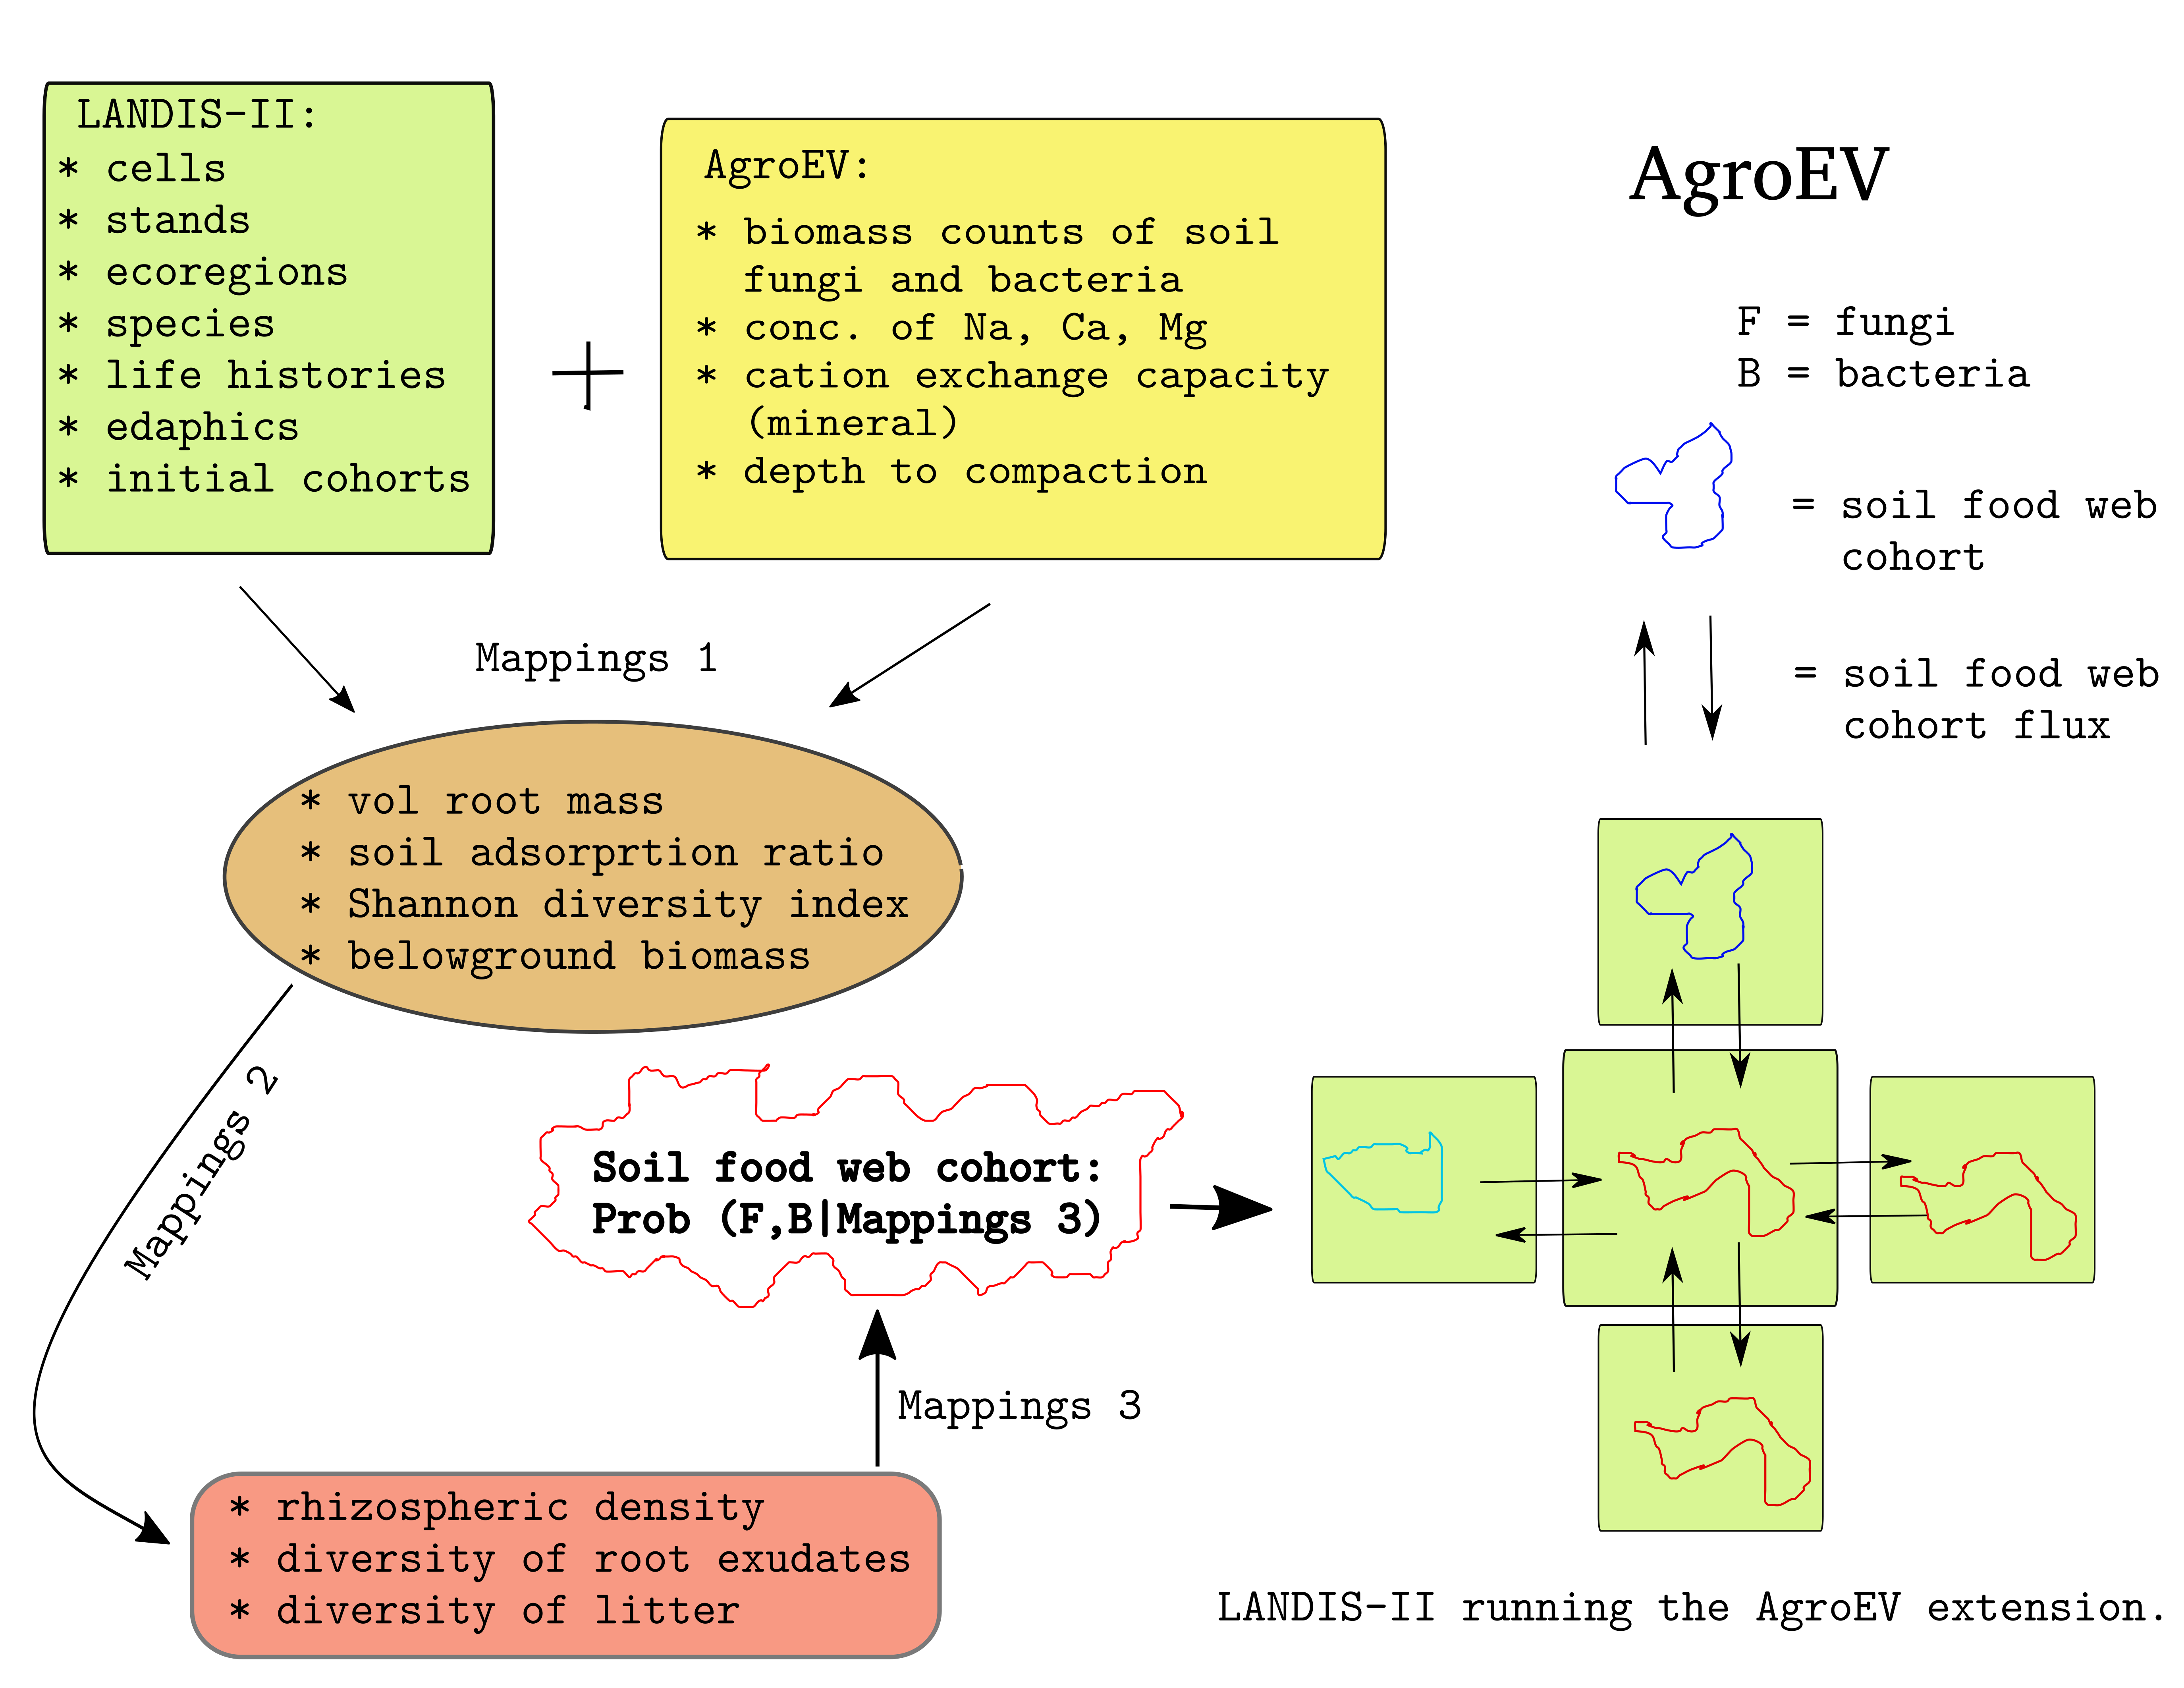
\includegraphics[scale = 0.60]{Ch4_AgroEV/graphics/AgroEV_doc.png}
    \caption{Concept sketch of the AgroEV extension for LANDIS-II.}
    \label{fig:}
  \end{center}
\end{figure}

\newpage
\subsection{Model Construction}
\todo{complete and fill}
\begin{outline}[enumerate]
\1 Use of the LANDIS-II architecture \citep{scheller_design_2007}
\1 Use of standard protocols for simulation model building, verification, and validation \citep{haefner_modeling_2005, law_simulation_2006}
\1 Use of best-practice software engineering plus standard operating procedures for QAQC to produce well-documented C\# code. Best practices and QAQC protocols include the use of GitHub for revision and change control, external code review, unit testing, and work logs. 
\1  
\end{outline}
 

 \label{chap:AgroEV}
 
 
\chapter{Applications of the AgroEV Extension}
 \todo{ Fill out all sections of this outline  }

\section{Background}

\section{Questions}
\begin{outline}
\1 What are the key spatial, temporal, ecological, and biological state variables that define the major successional stages of the Mayan successionally developed agroecosystem?
\1 What are the density distributions of the agroecological mutualism state variables for the Mayan successionally developed agroecosystem?
\1 What is the relationship between soil food webs and the major successional stages of the Mayan successionally developed agroecosystem?
\1 What is the relationship between agroecological mutualism and agricultural disturbance regimes based on the Mayan successionally developed agroecosystem model?
\end{outline}



\section{Hypotheses}
\begin{outline}
\1 The agricultural practices of the Lowland Maya during their Classical Period imposed a disturbance regime on the Yucat\'{a}n Peninsula that created a robust, resilient, and adaptive successionally developed agroecosystem; a verifiable example of agroecological mutualism


\end{outline}


\section{Aims and Objectives}
\begin{outline}
\1 Evaluate landscape-scale agroecological patterns can generate virtuous ecological processes for the sustainable production of food
\1 Build a series of agricultural management scenario-based LANDIS-II models that explore the relationships between landscape spatio-temporal patterns, agricultural disturbance regimes, soil food web classes, soil organic carbon dynamics, and succession.
\1 Design a set of LANDIS-II simulation experiments to test the effects of different agricultural disturbance regime patterns on agroecological mutualism processes
\1 Qualitatively assess soil biota (bacteria, fungi, protozoa, nematodes) for the major successional stages of the Mayan successionally developed agroecosystem
\1 Build a LANDIS-II model of the Mayan successionally developed agroecosystem.

\end{outline}



\section{Methods}

 \label{chap:Apps}

 
 
%----------------------------
% APPENDICES
%--------------------------------
\startappendices
 \appendix{A Few Definitions of Sustainable Agriculture}
  \section{The US Congress Idea}
\noindent Sec. 3103. Definitions.\\
(19) The term "sustainable agriculture" means an integrated system of plant and animal production practices having a site-specific application that will, over the long-term —
(A) satisfy human food and fiber needs;\\
(B) enhance environmental quality and the natural resource base upon which the agriculture economy depends;\\
(C) make the most efficient use of nonrenewable resources and on-farm resources and integrate, where appropriate, natural biological cycles and controls;\\
(D) sustain the economic viability of farm operations; and\\
(E) enhance the quality of life for farmers and society as a whole.\footnote{7 U.S.C. \S 3103(19)}


\section{The USDA Idea}
\noindent Sustainable agriculture is "a way of practicing agriculture which seeks to optimize skills and technology to achieve long-term stability of  the agricultural enterprise, environmental protection, and consumer safety. It is achieved through management strategies which help the producer select hybrids and varieties, soil conserving cultural practices, soil fertility programs, and pest management programs. The goal of sustainable agriculture is to minimize adverse impacts to the immediate and off-farm environments while providing a sustained level of production and profit. Sound resource conservation is an integral part of the means to achieve sustainable agriculture."\footnote{United States Department of Agriculture (USDA) Natural Resource Conservation Service (NRCS) General Manual (180-GM, Part 407)} 


\section{The EU Idea (the 'Evergreen Revolution')}
\noindent Sustainable agriculture aims to:\\
Produce safe and healthy food;\\
Conserve natural resources;\\
Ensure economic viability of farmlands;\\
Deliver services for the ecosystem and for people (biodiversity, soil conservation, nutrient storage, carbon storage);\\
Manage the countryside (preserve habitats and landscape beauty); \\
Improve quality of life in farming areas;\\
Ensure animal welfare\footnote{"Sustainable agriculture for the future we want"; EU Commissions on (1) Development and Cooperation, and (2) Agriculture and Rural Development, 2012}


\section{The Union of Concerned Scientists Idea}
\noindent "Sustainable agriculture does not mean a return to either the low yields or poor farmers that characterized the 19th century. Rather, sustainability builds on current agricultural achievements, adopting a sophisticated approach that can maintain high yields and farm profits without undermining the resources on which agriculture depends."\footnote{"Sustainable Agriculture - A New Vision"; Union of Concerned Scientists, 1999}  




  \label{app:defs}
 
 
  
%----------------------------------
% BIBLIOGRAPHY
%-----------------------------------  
 \startbibliography
 \begin{singlespace} % Bibliography must be single spaced
  \bibliographystyle{/usr/local/share/texmf/tex/latex/apacite/apacite}
  \bibliography{/home/bruce/Desktop/BibTex/My_Library_20170125}
 \end{singlespace}




%-----------------------------------------------------
% (Separate-submission) ABSTRACT
% -------------------------------------------------------
% An external Abstract that can be printed at the end of the document, 
% for separate submission, if needed.

%\startextabstractpage
%{The Title of Your Dissertation}{Your Name}{Chair: Albert Einstein}
%\textit{This template conforms to University of Michigan abstract and dissertation format guidelines as of September 2008. It is an update to a template that has been floating around among grad students here for about 20 years. The main components are the thesis.tex file and the rac.sty file, the latter of which should not need any modification. If BibTeX is used (and for a dissertation, it should be), then References.bib is also needed. If a list of acronyms is desired, make all additions in abbr.tex and read acronym.pdf on ctan.org for details on how to call them in the text. Other files in this template that may be helpful, but don't necessarily need to be used include a style file that formats your bibliography in AGU format (agu04.bst) and a style file that allows you to use abbreviations for journal names (aas\_macros.sty) when typing out the bibliography. This will be necessary if you grab BibTeX information from places like the NASA ADS, which sometimes uses journal name abbreviations. It is useful to separate chapters into their own subfolders, with each folder containing the chapter's .tex file as well as all associated figures. For the figures, just call the name of the file, without the suffix (i.e., includegraphics\{Chap5/LabSetup\}) and the graphicx package will figure out what type of file it is. To compile to pdf, some format other than .eps must be used with the figures. To compile to ps, the figures need to be in ps or eps. If using \LaTeX\, in a Windows environment, there are several different editors and programs that can be used. One set that is known to work well is the following, which can each be found with a simple web search and which should be installed in this order: a Perl distribution such as ActivePerl, a \TeX\, distribution such as MikTex, a \LaTeX\, editor such as TeXnicCenter, a postscript interpreter like Ghostscript, and a postscript viewer like GSView. I included a few pages of sample code in chapter 2 to help you get started, including code for writing equations, citations, abbreviations, tables, and calling graphics. Always be sure to compile your thesis.tex file a couple of times to get the references and page numbering updated.} Good luck. -jg

%\label{ExtAbstract}




%------------------------
% END DOCUMENT
%--------------------------
\end{document}
